\begin{frame}{Congestion Control}
    \begin{center}
        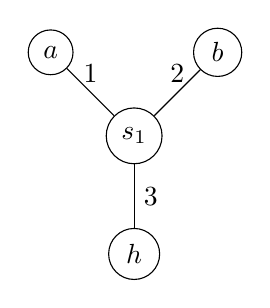
\begin{tikzpicture}[node distance={15mm},main/.style = {draw, circle}]
            \node[main] (s) {$s_1$};
            \node[main] (h) [below of=s] {$h$};
            \node[main] (a) [above left of=s]{$a$};
            \node[main] (b) [above right of=s]{$b$};
            \draw (a) --  node[above]{1}(s);
            \draw (b) --  node[above]{2}(s);
            \draw (s) --  node[right]{3}(h);
        \end{tikzpicture}
    \end{center}
    Consider a network where wish to forward traffic from $a$ and $b$ to $c$, while limiting the traffic on link 3 so that
    at any moment there must be at most one packet traversing this link.
\end{frame}

\begin{frame}
    \begin{center}
        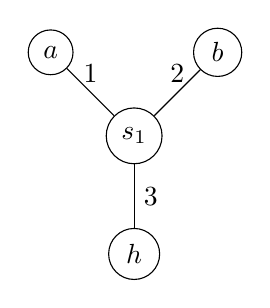
\begin{tikzpicture}[node distance={15mm},main/.style = {draw, circle}]
            \node[main] (s) {$s_1$};
            \node[main] (h) [below of=s] {$h$};
            \node[main] (a) [above left of=s]{$a$};
            \node[main] (b) [above right of=s]{$b$};
            \draw (a) --  node[above]{1}(s);
            \draw (b) --  node[above]{2}(s);
            \draw (s) --  node[right]{3}(h);
        \end{tikzpicture}
    \end{center}
    We define events $a,b$ representing the forwarding of a packet from
    1 to 3 and 2 to 3 respectively.
    We define an event $c$ when congestion is detected on link 3 (at least two packets are being traversed through the link).
    For this network, we can define an event structure $\mathrm{E}$
    with an empty conflict relation and an enabling relation the least
    one for which we have:
    \begin{align*}
        \e \vdash a, \e \vdash b, \s{a,b} \vdash c
    \end{align*}
\end{frame}

\begin{frame}
    \begin{center}
        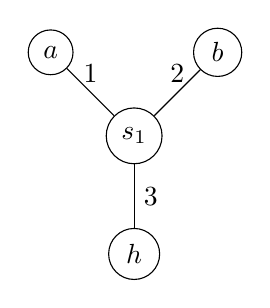
\begin{tikzpicture}[node distance={15mm},main/.style = {draw, circle}]
            \node[main] (s) {$s_1$};
            \node[main] (h) [below of=s] {$h$};
            \node[main] (a) [above left of=s]{$a$};
            \node[main] (b) [above right of=s]{$b$};
            \draw (a) --  node[above]{1}(s);
            \draw (b) --  node[above]{2}(s);
            \draw (s) --  node[right]{3}(h);
        \end{tikzpicture}
    \end{center}
    Event structure of this network has configurations of the form:
    \begin{center}
        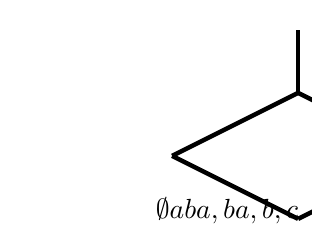
\begin{tikzpicture}[scale=0.8]
            \crd{0}{0}{$\emptyset$}
            \crd[above]{-2}{1}{$\s{a}$}
            \crd[above]{2}{1}{$\s{b}$}
            \crd[left]{0}{2}{$\s{a,b}$}
            \crd[left]{0}{3}{$\s{a,b,c}$}
            \draw [ultra thick] (0,0) -- (-2,1);
            \draw [ultra thick] (0,0) -- (2,1);
            \draw [ultra thick] (-2,1) -- (0,2);
            \draw [ultra thick] (2,1) -- (0,2);
            \draw [ultra thick] (0,2) -- (0,3);
        \end{tikzpicture}
    \end{center}
\end{frame}

\begin{frame}
    \begin{center}
        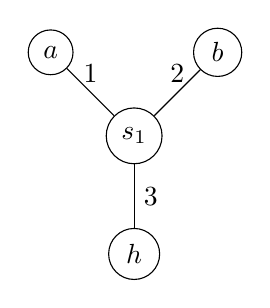
\begin{tikzpicture}[node distance={15mm},main/.style = {draw, circle}]
            \node[main] (s) {$s_1$};
            \node[main] (h) [below of=s] {$h$};
            \node[main] (a) [above left of=s]{$a$};
            \node[main] (b) [above right of=s]{$b$};
            \draw (a) --  node[above]{1}(s);
            \draw (b) --  node[above]{2}(s);
            \draw (s) --  node[right]{3}(h);
        \end{tikzpicture}
        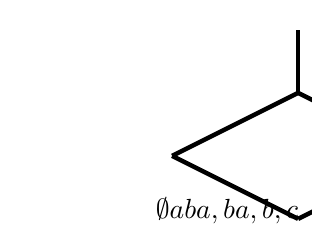
\begin{tikzpicture}[scale=0.8]
            \crd{0}{0}{$\emptyset$}
            \crd[above]{-2}{1}{$\s{a}$}
            \crd[above]{2}{1}{$\s{b}$}
            \crd[left]{0}{2}{$\s{a,b}$}
            \crd[left]{0}{3}{$\s{a,b,c}$}
            \draw [ultra thick] (0,0) -- (-2,1);
            \draw [ultra thick] (0,0) -- (2,1);
            \draw [ultra thick] (-2,1) -- (0,2);
            \draw [ultra thick] (2,1) -- (0,2);
            \draw [ultra thick] (0,2) -- (0,3);
        \end{tikzpicture}
    \end{center}
    Assume that we consider $\sigma = \s{a,bc}$ as a counterexample.
    We may declare $C(a,b) = \F$ as a cause of $\sigma \in \mathcal{F}(\mathrm{E})$.
\end{frame}

\begin{frame}
    \begin{center}
        \begin{tikzpicture}[node distance=20mm]
            \node[b] (eabc) {$EN(\s{a,b},c)$};
            \node[r] (ebc) [above left of=eabc] {$EN(\s{b},c)$};
            \node[r] (eac) [left of=ebc] {$EN(\s{a},c)$};
            \node[r] (eec) [above right of=eac,left of=ebc] {$EN(\e,c)$};
            \node[r] (mac) [above left of=eec] {$M(\s{a},c)$};
            \node[r] (mbc) [above right of=eec] {$M(\s{b},c)$};
            \node[r] (mec) [above left of=mbc] {$M(\e,c)$};
            \node[b] (mabc) [above right of=eabc] {$M(\s{a,b},c)$};
            \node[r] (cab) [above left of=mabc] {$C(a,b)$};
            \draw [->] (mec) -- (mac);
            \draw [->] (mec) -- (eec);
            \draw [->] (mec) -- (mbc);
            \draw [->] (mac) -- (eac);
            \draw [->] (mbc) -- (ebc);
            \draw [->] (mbc) -| (mabc);
            \draw [->] (eec) -- (eac);
            \draw [->] (eec) -- (ebc);
            \draw [->] (eac) -- (eabc);
            \draw [->] (ebc) -- (eabc);
            \draw [->] (cab) -- (eabc);
            \draw [->] (cab) -- (mabc);
            \draw [->] (mabc) edge (eabc);
            \draw [->] (mec) -- (2,5.6) -- (mabc);
            \draw [->] (mac) -- (-3,6) -- (3,6) -- (3,2.5) -- (mabc);
        \end{tikzpicture}
    \end{center}
\end{frame}

\begin{frame}
    \begin{center}
        \begin{tikzpicture}[node distance=20mm]
            \node[b] (eabc) {$EN(\s{a,b},c)$};
            \node[r] (ebc) [above left of=eabc] {$EN(\s{b},c)$};
            \node[r] (eac) [left of=ebc] {$EN(\s{a},c)$};
            \node[r] (eec) [above right of=eac,left of=ebc] {$EN(\e,c)$};
            \node[r] (mac) [above left of=eec] {$M(\s{a},c)$};
            \node[r] (mbc) [above right of=eec] {$M(\s{b},c)$};
            \node[r] (mec) [above left of=mbc] {$M(\e,c)$};
            \node[b] (mabc) [above right of=eabc] {$M(\s{a,b},c)$};
            \node[o] (cab) [above left of=mabc] {$C(a,b)$};
            \draw [->] (mec) -- (mac);
            \draw [->] (mec) -- (eec);
            \draw [->] (mec) -- (mbc);
            \draw [->] (mac) -- (eac);
            \draw [->] (mbc) -- (ebc);
            \draw [->] (mbc) -| (mabc);
            \draw [->] (eec) -- (eac);
            \draw [->] (eec) -- (ebc);
            \draw [->] (eac) -- (eabc);
            \draw [->] (ebc) -- (eabc);
            \draw [->] (cab) -- (eabc);
            \draw [->] (cab) -- (mabc);
            \draw [->] (mabc) edge (eabc);
            \draw [->] (mec) -- (2,5.6) -- (mabc);
            \draw [->] (mac) -- (-3,6) -- (3,6) -- (3,2.5) -- (mabc);
        \end{tikzpicture}
    \end{center}
\end{frame}

\begin{frame}
    \begin{center}
        \begin{tikzpicture}[node distance=20mm]
            \node[o] (eabc) {$EN(\s{a,b},c)$};
            \node[r] (ebc) [above left of=eabc] {$EN(\s{b},c)$};
            \node[r] (eac) [left of=ebc] {$EN(\s{a},c)$};
            \node[r] (eec) [above right of=eac,left of=ebc] {$EN(\e,c)$};
            \node[r] (mac) [above left of=eec] {$M(\s{a},c)$};
            \node[r] (mbc) [above right of=eec] {$M(\s{b},c)$};
            \node[r] (mec) [above left of=mbc] {$M(\e,c)$};
            \node[o] (mabc) [above right of=eabc] {$M(\s{a,b},c)$};
            \node[b] (cab) [above left of=mabc] {$C(a,b)$};
            \draw [->] (mec) -- (mac);
            \draw [->] (mec) -- (eec);
            \draw [->] (mec) -- (mbc);
            \draw [->] (mac) -- (eac);
            \draw [->] (mbc) -- (ebc);
            \draw [->] (mbc) -| (mabc);
            \draw [->] (eec) -- (eac);
            \draw [->] (eec) -- (ebc);
            \draw [->] (eac) -- (eabc);
            \draw [->] (ebc) -- (eabc);
            \draw [->] (cab) -- (eabc);
            \draw [->] (cab) -- (mabc);
            \draw [->] (mabc) edge (eabc);
            \draw [->] (mec) -- (2,5.6) -- (mabc);
            \draw [->] (mac) -- (-3,6) -- (3,6) -- (3,2.5) -- (mabc);
        \end{tikzpicture}
    \end{center}
\end{frame}

\begin{frame}
    \begin{center}
        \begin{tikzpicture}[node distance=20mm]
            \node[r] (eabc) {$EN(\s{a,b},c)$};
            \node[r] (ebc) [above left of=eabc] {$EN(\s{b},c)$};
            \node[r] (eac) [left of=ebc] {$EN(\s{a},c)$};
            \node[r] (eec) [above right of=eac,left of=ebc] {$EN(\e,c)$};
            \node[r] (mac) [above left of=eec] {$M(\s{a},c)$};
            \node[r] (mbc) [above right of=eec] {$M(\s{b},c)$};
            \node[r] (mec) [above left of=mbc] {$M(\e,c)$};
            \node[r] (mabc) [above right of=eabc] {$M(\s{a,b},c)$};
            \node[b] (cab) [above left of=mabc] {$C(a,b)$};
            \draw [->] (mec) -- (mac);
            \draw [->] (mec) -- (eec);
            \draw [->] (mec) -- (mbc);
            \draw [->] (mac) -- (eac);
            \draw [->] (mbc) -- (ebc);
            \draw [->] (mbc) -| (mabc);
            \draw [->] (eec) -- (eac);
            \draw [->] (eec) -- (ebc);
            \draw [->] (eac) -- (eabc);
            \draw [->] (ebc) -- (eabc);
            \draw [->] (cab) -- (eabc);
            \draw [->] (cab) -- (mabc);
            \draw [->] (mabc) edge (eabc);
            \draw [->] (mec) -- (2,5.6) -- (mabc);
            \draw [->] (mac) -- (-3,6) -- (3,6) -- (3,2.5) -- (mabc);
        \end{tikzpicture}
    \end{center}
\end{frame}

\begin{frame}
    \begin{align*}
        M & \vDash EN(\e,a)       = \T              &
        M & \vDash[C(a,b)\la T] EN(\e,a)       = \T   \\
        M & \vDash EN(\s{b},a)    = \T              &
        M & \vDash[C(a,b)\la T] EN(\s{b},a)    = \T   \\
        M & \vDash EN(\s{c},a)    = \T              &
        M & \vDash[C(a,b)\la T] EN(\s{c},a)    = \T   \\
        M & \vDash EN(\s{b,c},a)  = \T              &
        M & \vDash[C(a,b)\la T] EN(\s{b,c},a)  = \T   \\
        M & \vDash EN(\e,b)       = \T              &
        M & \vDash[C(a,b)\la T] EN(\e,b)       = \T   \\
        M & \vDash EN(\s{a},b)    = \T              &
        M & \vDash[C(a,b)\la T] EN(\s{a},b)    = \T   \\
        M & \vDash EN(\s{c},b)    = \T              &
        M & \vDash[C(a,b)\la T] EN(\s{c},b)    = \T   \\
        M & \vDash EN(\s{a,c},b)  = \T              &
        M & \vDash[C(a,b)\la T] EN(\s{a,c},b)  = \T   \\
        M & \vDash EN(\e,c)       = \F              &
        M & \vDash[C(a,b)\la T] EN(\e,c)       = \F   \\
        M & \vDash EN(\s{a},c)    = \F              &
        M & \vDash[C(a,b)\la T] EN(\s{a},c)    = \F   \\
        M & \vDash EN(\s{b},c)    = \F              &
        M & \vDash[C(a,b)\la T] EN(\s{b},c)    = \F   \\
        M & \vDash EN(\s{a,b},c)  = \T              &
        M & \vDash[C(a,b)\la T] EN(\s{a,b},c)  = \F   \\
    \end{align*}
\end{frame}
\begin{frame}
    \begin{center}
        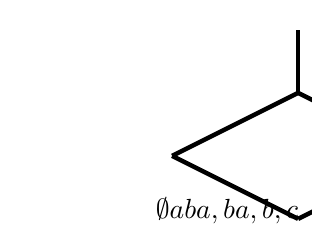
\begin{tikzpicture}[scale=0.8]
            \crd{0}{0}{$\emptyset$}
            \crd[above]{-2}{1}{$\s{a}$}
            \crd[above]{2}{1}{$\s{b}$}
            \crd[left]{0}{2}{$\s{a,b}$}
            \crd[left]{0}{3}{$\s{a,b,c}$}
            \draw [ultra thick] (0,0) -- (-2,1);
            \draw [ultra thick] (0,0) -- (2,1);
            \draw [ultra thick] (-2,1) -- (0,2);
            \draw [ultra thick] (2,1) -- (0,2);
            \draw [ultra thick] (0,2) -- (0,3);
        \end{tikzpicture} 
        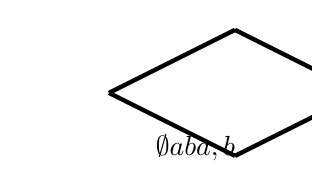
\begin{tikzpicture}[scale=0.8]
            \crd{0}{0}{$\emptyset$}
            \crd[above]{-2}{1}{$\s{a}$}
            \crd[above]{2}{1}{$\s{b}$}
            \crd[left]{0}{2}{$\s{a,b}$}
            \draw [ultra thick] (0,0) -- (-2,1);
            \draw [ultra thick] (0,0) -- (2,1);
            \draw [ultra thick] (-2,1) -- (0,2);
            \draw [ultra thick] (2,1) -- (0,2);
        \end{tikzpicture} 
    \end{center}
\end{frame}